\documentclass[11pt]{article}
\usepackage[T1]{fontenc}
\usepackage[utf8]{inputenc}
\usepackage{lmodern,microtype,amsmath,amssymb,amsthm,mathtools}
\usepackage[margin=30mm]{geometry}
\usepackage{tikz}
\usetikzlibrary{arrows.meta}
\usepackage{xcolor,xurl}
\usepackage[unicode,colorlinks=true,linkcolor=blue!45!black,urlcolor=blue!55!black,citecolor=green!35!black]{hyperref}
\setlength{\emergencystretch}{2em}
\numberwithin{equation}{section}
\newtheorem{theorem}{Theorem}[section]
\newtheorem{proposition}[theorem]{Proposition}
\newtheorem{lemma}[theorem]{Lemma}
\newtheorem{corollary}[theorem]{Corollary}
\theoremstyle{remark}\newtheorem{remark}[theorem]{Remark}
\newcommand{\coefle}{\preccurlyeq}
\newcommand{\coefge}{\succcurlyeq}
\newcommand{\abscoef}[1]{\left|#1\right|_{\rm coef}}
\title{Uniform spectral bounds for local Casimir sources}
\author{}\date{}
\begin{document}\maketitle
\begin{abstract}
We estimate the homogeneous four-variable polynomial of the full finite
Casimir resolvent on the entire real spectral interval. Its decreasing
matrix paths partition into a central sector and two one-sided sectors.
For arbitrary face phases, we prove uniform exponential upper bounds
in terms of an explicitly normalized triangle entropy. The central
bound follows from exact cofactor interpolation at the physical nodes.
The one-sided bound retains both unused spectral products and the signs
inside an interval continuant; its two endpoint optimization has an
explicit solution. The estimates include even and odd levels, the
odd central-skipping term, and face variables fixed exactly at zero.
They do not require a nonzero complex asymptotic or identify a volume.
\end{abstract}

\section{The local bounds}
The variables of a local face polynomial have a prescribed order:
\(x,y\) are the outer variables, \(b\) the input middle variable, and
\(c\) the output middle variable. Variables shared by different boxes
must later be identified. This paper estimates one actual polynomial
before that shared extraction. The estimates hold for all phases of
the four variables, rather than only at their positive real values.

Fix an integer \(N\ge3\), and put
\[
 d=N-1,\quad m=\lfloor N/2\rfloor,\quad
 \theta=\pi/N,\quad q=e^{i\theta},\quad Q=q^2.
\]
The finite Fourier theorem in \cite[Proposition 4.1 and
equations (4.4)--(4.5)]{FinitePaper} identifies the physical pair Casimir
\(\Omega\), one \(N\)-dimensional residue block at a time, with the
polynomial operator specified in Section~\ref{lc:source}. The identification
uses a finite Fourier transform, a transpose and a diagonal change of basis;
it is stated precisely below. It also proves \(\chi_N(\Omega)=0\), where
\(\chi_N(z)=2T_N(z/2)+2\) and \(T_N(\cos t)=\cos Nt\).
The full resolvent numerator is the polynomial
\[
 V_N(\sigma;\Omega)
       =\frac{\chi_N(\sigma)-\chi_N(\Omega)}{\sigma-\Omega}.
\]
The fraction is polynomial division, not an inverse at a spectral root.
Its degree in \(\sigma\) is \(d\); it retains the first derivatives at
double roots as well as the values at distinct roots.

Write \(H_V(x,b,c,y;\sigma)\) for its homogeneous face polynomial.
Section~\ref{lc:source} gives a division-free definition and fixes its
sign. A decreasing path from row \(j\) to row \(i\) contributes the
middle monomial \(b^ic^{d-j}\). When \(N=2m\), its central sector
has \(i\le m-1,j\ge m\); when \(N=2m+1\), it has \(i\le m,j\ge m\).
The left sector has \(j<m\); the right consists of the remaining
paths above the central cut. Denote these three polynomials by
\(H_{V,\mathrm C},H_{V,\mathrm L},H_{V,\mathrm R}\).
This is a partition of the full numerator paths, not a new spectral
operator.

Set
\[
 \mathcal B(t)=-\int_0^t\log|2\sin v|\,dv,\qquad
 e(a)=\frac{\mathcal B(\pi a)+\mathcal B(\pi/2-\pi a)}{\pi},
 \quad 0\le a\le\tfrac12.
\]
For nonnegative \(w_1,w_2,w_3\), not all zero, define
\begin{equation}\label{lc:entropy}
 \mathcal Q(w_1,w_2,w_3)=
 \max_{\substack{a_i\ge0,\ \sum_i a_i=1/2\\a_i=0\ {\rm if}\ w_i=0}}
 \left\{\sum_i e(a_i)+\sum_{w_i>0}a_i\log w_i\right\}.
\end{equation}
A variable fixed at zero has exactly zero load. It is never replaced
silently by a small positive radius. The logarithmic integrals are
finite at their endpoints. To fix their normalization, put
\(I=\int_0^{\pi/2}\log\sin t\,dt\). Reflection and the double-angle
formula give \(2I=I-(\pi/2)\log2\). Hence
\(\mathcal B(0)=\mathcal B(\pi/2)=0\), and \(e(0)=e(1/2)=0\).

In the theorem the lowercase letters denote nonnegative moduli.
For \(x+y>0\), put
\begin{equation}\label{lc:rates}
\begin{aligned}
 Q_b&=\mathcal Q(x,b,y),&Q_c&=\mathcal Q(x,c,y),&X&=Q_b+Q_c,\\
 A_{\mathrm L}&=\max\{\log c,Q_b+\tfrac12\log c\}&&(c>0),\\
 A_{\mathrm R}&=\max\{\log b,Q_c+\tfrac12\log b\}&&(b>0).
\end{aligned}
\end{equation}
If \(c=0\), the left polynomial is zero and its rate is interpreted
as \(-\infty\); the same convention applies on the right when \(b=0\).

\begin{theorem}[Uniform local sector bounds]\label{lc:main}
Fix nonnegative face moduli \((x,b,c,y)\) with \(x+y>0\). For
\(s=\mathrm C,\mathrm L,\mathrm R\),
\begin{equation}\label{lc:main-rate}
 \limsup_{N\to\infty}\frac1N
 \log\sup_{\substack{\sigma\in[-2,2]\\
 |X_0|=x,\ |B_0|=b,\ |C_0|=c,\ |Y_0|=y}}
 |H_{V,s}(X_0,B_0,C_0,Y_0;\sigma)|
 \le
 \begin{cases}
 X&s=\mathrm C,\\
 A_{\mathrm L}&s=\mathrm L,\\
 A_{\mathrm R}&s=\mathrm R.
 \end{cases}
\end{equation}
The limit superior is over all integer levels, including both parities
and composite levels. The statement is uniform when the zero pattern
is fixed and every nonzero modulus varies in a fixed compact subset
of \((0,\infty)\). Thus, for every \(\varepsilon>0\), there is one
threshold \(N_0\) on such a compact set for which the indicated rate
plus \(\varepsilon\) bounds the normalized logarithm at every \(N\ge N_0\).
\end{theorem}

The supremum precedes the limit, so sampled spectral zeros are included.
The proof never divides a finite numerator by such a zero, and never
replaces a negative tail coefficient by its absolute value inside the
recurrence.

The admissible vertex with load \(1/2\) on \(b\) gives
\begin{equation}\label{lc:spectator}
 \mathcal Q(x,b,y)\ge\tfrac12\log b\quad(b>0),\qquad
 \max\{X,A_{\mathrm L},A_{\mathrm R}\}=\max\{X,\log b,\log c\},
\end{equation}
with undefined logarithms omitted. Each mixed expression in
\eqref{lc:rates} is at most \(X\). This identifies the full local
spectator bound, but does not identify an optimized collection of
local bounds with a shared coefficient.

\section{The exact polynomial and its path partition}\label{lc:source}
We import only the finite operator identification from \cite{FinitePaper}.
The matrix needed in the estimates is explicit. On \(1,z,\ldots,z^d\),
let
\begin{equation}\label{lc:banded}
 \mathsf C z^j=2\cos((2j+1)\theta)z^j
       -s_j^2(x+y)z^{j-1}-s_js_{j-1}xy\,z^{j-2},
 \qquad s_j=2\sin(j\theta).
\end{equation}
Negative powers vanish because \(s_0=0\). In the finite Fourier theorem
\(\mathsf C=-T\). To specify the imported identification, let
\(\Omega_s\) be the block of the physical pair operator on
\[
 e_u\otimes e_{[s-u]_N},\qquad 0\le u<N,\qquad 0\le s<N.
\]
Here \(e_0,\ldots,e_d\) is its standard one-strand basis, and
\([v]_N\) is the representative in \(\{0,\ldots,N-1\}\).
For \(y\ne0\), specialize \(x=Q^{s+1}y\), set
\(\zeta_u=-q^{-1}xQ^{-u}\), and define
\(\mathsf E_{uj}=\zeta_u^j\), \(G_{uu}=q^{du}\). Then
\begin{equation}\label{lc:residue-adapter}
 \mathsf E\mathsf C\mathsf E^{-1}
                     =G^{-1}\Omega_s^{\mathsf T}G.
\end{equation}
The \(N\) blocks form the \(N^2\)-dimensional pair space. The identity
includes their nilpotent parts, not just eigenvalues. The face
polynomial retains independent \(x,y\); its specialized values recover
the matrix entries by the adapter in \cite[equation (4.5)]{FinitePaper}.
If \(f(\mathsf C)_{ij}\) is the coefficient from \(z^j\)
to \(z^i\), the homogeneous polynomial is
\[
 H_f(x,b,c,y)=\sum_{0\le i\le j\le d}f(\mathsf C)_{ij}b^ic^{d-j}.
\]
Its entries are polynomials in \(x,y\), and its total face degree is \(d\).

Set
\begin{equation}\label{lc:diagonal}
 \sigma=-2-u,\qquad a_j=2+2\cos((2j+1)\theta),\qquad
 \alpha_j=a_j+u,\qquad A=x+y,\quad P=xy.
\end{equation}
The triangular matrix \(\mathsf M=2I+\mathsf C+uI\) has diagonal
\(\alpha_j\), and lowering entries \(-s_j^2A\), \(-s_js_{j-1}P\).
Its diagonal product is \((-1)^N\chi_N(-2-u)\). Consequently
\begin{equation}\label{lc:adjugate}
 \mathcal P_N(x,b,c,y;u):=(-1)^dH_V(x,b,c,y;-2-u)
       =\sum_{i\le j}(\operatorname{adj}\mathsf M)_{ij}b^ic^{d-j}.
\end{equation}
The identity follows first where \(\mathsf M\) is invertible and then
by polynomial equality, including every singular spectral value.

Expand its triangular inverse by the strictly lowering part and
multiply by all diagonal factors. A path \(j\to i\) uses steps of length
one or two. Its weight is the product of \(s_r^2A\) for a step
\(r\to r-1\), \(s_rs_{r-1}P\) for a step \(r\to r-2\), and
\(\alpha_r\) for precisely the rows it does not visit.
The middle monomial \(b^ic^{d-j}\) completes its term.
This proves the path rule, including the case of a zero unused factor.

Partition \(\mathcal P_N=\mathcal P_{\mathrm C}+\mathcal P_{\mathrm L}
+\mathcal P_{\mathrm R}\) by the sectors in the introduction.
Their common sign relative to \(H_V\) does not affect modulus bounds.
Every sector has spectral degree at most \(d\). At \(u=0\), every
path weight is nonnegative. At odd \(N\), a path missing the middle
row has its unused factor \(a_m=0\).

\begin{figure}[ht]
\centering
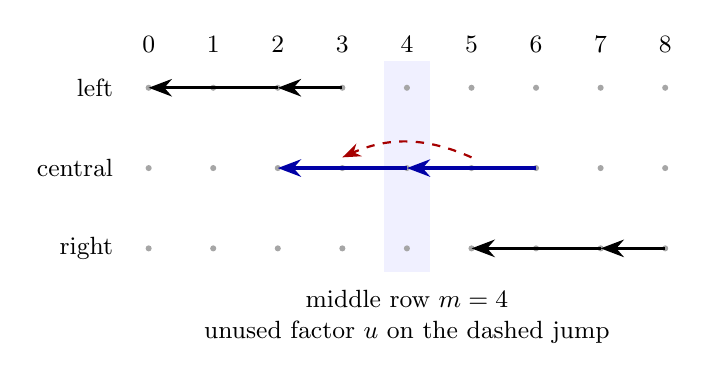
\begin{tikzpicture}[x=.82cm,y=.68cm,>=Stealth,font=\small]
 \fill[blue!6] (3.65,-.45) rectangle (4.35,3.5);
 \foreach \j in {0,...,8}{
  \node at (\j,3.8){\(\j\)};
  \foreach \h in {0,1.5,3}{\fill[black!35] (\j,\h) circle(1.1pt);}
 }
 \draw[->,very thick] (3,3)--(2,3);
 \draw[->,very thick] (2,3)--(0,3);
 \node[left] at (-.4,3){left};
 \draw[->,very thick,blue!65!black] (6,1.5)--(4,1.5);
 \draw[->,very thick,blue!65!black] (4,1.5)--(2,1.5);
 \draw[->,thick,dashed,red!65!black] (5,1.7) to[bend right=24] (3,1.7);
 \node[left] at (-.4,1.5){central};
 \draw[->,very thick] (8,0)--(7,0);
 \draw[->,very thick] (7,0)--(5,0);
 \node[left] at (-.4,0){right};
 \node[below,align=center] at (4,-.6){middle row \(m=4\)\\
           unused factor \(u\) on the dashed jump};
\end{tikzpicture}
\caption{The partition at the illustrative odd level \(N=9\).
A central path may visit row \(m\), or skip it by \(m+1\to m-1\).
The skipped row contributes its unused factor \(u\), retained in the
exact central polynomial even though it vanishes at \(u=0\).}
\label{lc:path-figure}
\end{figure}

\subsection{Cleared cofactors}
Let \(R_j(b;u)\) be the determinant obtained from the block of
\(\mathsf M\) on rows \(0,\ldots,j\) by replacing its last row with
\((1,b,\ldots,b^j)\). Its path expansion gives
\begin{equation}\label{lc:R-recurrence}
\begin{split}
 R_0&=1,\qquad R_{-1}=R_{-2}=0,\\
 R_j(b;u)&=b^j\prod_{r<j}\alpha_r+s_j^2A R_{j-1}(b;u)
                +s_js_{j-1}\alpha_{j-1}P R_{j-2}(b;u).
\end{split}
\end{equation}
The first term at \(j=0\) is the empty product one. Each \(R_j\)
has face degree \(j\) and spectral degree at most \(j\). Put
\[
 D_b=R_{m-1}(b;u),\qquad E_b=\alpha_{m-1}R_{m-2}(b;u),
\]
with \(E_b=0\) when \(m=1\). Subscripts \(b,c\) here denote substitution
of the middle variable, not differentiation.

\begin{lemma}[Exact central factors]\label{lc:central-factors}
At \(N=2m\),
\begin{equation}\label{lc:even-factor}
 \mathcal P_{\mathrm C}
 =s_m^2A D_bD_c+s_ms_{m-1}P(D_bE_c+E_bD_c).
\end{equation}
At \(N=2m+1\), with \(G_b=R_m(b;u)\),
\begin{equation}\label{lc:odd-factor}
 \mathcal P_{\mathrm C}=G_bG_c+u s_m^2P D_bD_c.
\end{equation}
Both are polynomial identities for every \(u\).
\end{lemma}
\begin{proof}
An even central path crosses the cut exactly once, by \(m\to m-1\),
\(m+1\to m-1\), or \(m\to m-2\). Their weights give the three
terms. Reflection \(r\mapsto d-r\) identifies upper and lower
cofactors: \(a_{d-r}=a_r\), and the reflected step products agree.
At odd level, paths visiting \(m\) split there to give \(G_bG_c\).
A path skipping it has the unique jump \(m+1\to m-1\), with weight
\(s_{m+1}s_mP=s_m^2P\); its unused diagonal is \(u\).
This proves the second term without dividing by \(u\).
\end{proof}

The same reflection interchanges the left and right sectors and \(b,c\).
A one-step at \(r\) reflects to one at \(N-r\), with \(s_{N-r}=s_r\);
a two-step reflects to one at \(N+1-r\), with product \(s_{r-1}s_r\).
It therefore suffices to estimate the left sector.

\section{Exact nodal control of the central sector}\label{lc:nodal}
For face polynomials, \(F\coefle G\) means that every coefficient of
\(G-F\) is nonnegative real. The symbol \(\abscoef F\) replaces each
coefficient by its modulus. Put \(J=\lfloor(N-1)/2\rfloor\).
The \(J+1\) distinct physical nodes in the \(u\) coordinate are
\[
                         u_a=-a_a,\qquad 0\le a\le J.
\]
They include zero at odd level, but not at even level.

\begin{lemma}[Nodal positivity and comparison]\label{lc:nodal-positive}
For every \(0\le j,a\le J\),
\[
                    0\coefle R_j(b;u_a)\coefle R_j(b;0).
\]
\end{lemma}
\begin{proof}
If \(j\le a\), every diagonal factor used in \eqref{lc:R-recurrence}
lies between zero and its value at \(u=0\); induction proves the claim.
If \(j>a\), the inhomogeneous term vanishes after row \(a\).
Every surviving path must visit row \(a\), so
\[
                    R_j(b;u_a)=K_{a,j}(u_a)R_a(b;u_a),
\]
where the interval continuant satisfies
\[
 K_{i,i}=1,\quad K_{i,i-1}=0,\quad
 K_{i,j}=s_j^2A K_{i,j-1}+s_js_{j-1}\alpha_{j-1}P K_{i,j-2}.
\]
Normalize \(q_r=K_{a,a+r}/\prod_{v=a+1}^{a+r}s_v^2\).
For \(r\ge2\), \(j=a+r\le J\), product-to-sum gives
\[
 a_{j-1}-a_a=-s_{j+a}s_{j-a-1},\qquad
 s_js_{j-1}-s_{j+a}s_{j-a-1}=s_as_{a+1}.
\]
All the indicated sines are nonnegative. Thus
\begin{equation}\label{lc:tail-node}
 q_0=1,\quad q_1=x+y,\quad
 q_r=(x+y)q_{r-1}-\gamma_rxyq_{r-2},\qquad
 \gamma_r=1-\frac{s_as_{a+1}}{s_js_{j-1}}\in[0,1].
\end{equation}
The identity
\[
 q_r-xq_{r-1}
 =y(q_{r-1}-xq_{r-2})+(1-\gamma_r)xyq_{r-2}
\]
proves simultaneous coefficientwise positivity, starting from
\(q_0=1,q_1-xq_0=y\). Also \(q_r\coefle(x+y)^r\).
At \(u=0\), the interval continuant contains this all-one-step term
and other nonnegative terms. Hence \(K_{a,j}(u_a)\coefle K_{a,j}(0)\).
The product \(K_{a,j}(0)R_a(b;0)\) is the subset of paths in \(R_j(b;0)\)
whose start is at or below \(a\) and which visit \(a\). This proves
the assertion without assuming positivity of the signed recurrence.
\end{proof}

\begin{lemma}[Exact interpolation bound]\label{lc:interpolation}
An absolute constant \(C\) gives, for \(j\le J\),
\begin{equation}\label{lc:cofactor-comparison}
 \abscoef{R_j(b;u)}\coefle C(1+\log N)R_j(b;0),\qquad -4\le u\le0.
\end{equation}
\end{lemma}
\begin{proof}
Each face coefficient is a polynomial in \(u\) of degree at most
\(j\le J\). This interpolation is not applied to the degree-\(d\)
full resolvent. Use \(z=-1-u/2\) and
\(\phi_k=(2k+1)\pi/N\), \(0\le k<N\).
For a polynomial \(p(z)\) of degree at most \(J\), discrete Fourier
inversion gives
\[
 p(\cos t)=\frac1N\sum_{k=0}^{N-1}D_J(t-\phi_k)p(\cos\phi_k),
 \qquad D_J(v)=\sum_{\ell=-J}^Je^{i\ell v}.
\]
The difference of any two retained modes has magnitude less than \(N\),
so its grid average is a Kronecker delta. Pairing equal cosine nodes
gives ordinary interpolation, with the unpaired point \(-1\) at odd \(N\).
Since
\[
 |D_J(v)|\le\min(2J+1,|\sin(v/2)|^{-1}),
\]
the normalized sum of absolute kernel values on any translate of the
grid is at most \(C(1+\log N)\). The two nearest points cost a constant;
successive distances \(k/N\) cost at most \(C/k\). Pairing cannot
increase this bound. Apply it to each coefficient and use
Lemma~\ref{lc:nodal-positive}.
\end{proof}

\begin{proposition}[Central polynomial comparison]\label{lc:central-comparison}
For an absolute \(C\) and every \(N\ge3\),
\begin{equation}\label{lc:central-coefficientwise}
 \abscoef{\mathcal P_{\mathrm C}(u)}
 \coefle C(1+\log N)^2\mathcal P_{\mathrm C}(0),\qquad -4\le u\le0.
\end{equation}
\end{proposition}
\begin{proof}
Apply \eqref{lc:cofactor-comparison} to the exact central factors.
The scalar factors \(|u|,|a_{m-1}+u|\) are at most four.
At even \(N\ge4\),
\[
 D_b(0)\coefge s_{m-1}^2(x+y)R_{m-2}(b;0),\qquad (x+y)^2\coefge2xy.
\]
The sine is uniformly bounded below. Thus either mixed term
\(xyD_b(0)R_{m-2}(c;0)\) is bounded coefficientwise by a constant
times \((x+y)D_b(0)D_c(0)\), already present at zero.
At odd levels,
\[
 G_b(0)\coefge s_m^2(x+y)D_b(0),\qquad
 G_b(0)G_c(0)\coefge2s_m^4xyD_b(0)D_c(0).
\]
Here \(s_m\) is bounded below, including \(N=3\).
The skipped-middle term is therefore controlled as well.
\end{proof}

\section{A signed interval transfer estimate}\label{lc:transfer}
This section bounds the signed recurrence. It is not a Perron estimate
for its entrywise absolute value. Parametrize the real interval by
\[
 \sigma=-2\cos(2\pi\delta),\qquad u=-4\sin^2(\pi\delta),
                    \qquad0\le\delta\le\tfrac12.
\]
For positive outer sum \(A=x+y\) and \(P=xy\ge0\), define
\begin{equation}\label{lc:continuous-coefficients}
\begin{aligned}
 a_\delta(t)&=4(\cos^2(\pi t)-\sin^2(\pi\delta)),\\
 \rho_\delta(t)&=A\sin(\pi t)+
   \sqrt{(x-y)^2\sin^2(\pi t)+4P\cos^2(\pi\delta)},\\
 \lambda_\delta(t)&=2\sin(\pi t)\rho_\delta(t).
\end{aligned}
\end{equation}
On each compact set of allowed moduli,
\begin{equation}\label{lc:endpoint-size}
 ct\le\rho_\delta(t)\le C,\qquad ct^2\le\lambda_\delta(t)\le C,
                          \qquad0<t\le\tfrac12,
\end{equation}
uniformly in \(\delta\).

\begin{lemma}[Uniform signed transfer]\label{lc:slow-transfer}
For every \(\varepsilon>0\), all sufficiently large \(N\) satisfy
\begin{equation}\label{lc:transfer-estimate}
 |K_{i,j}|\le
 \exp\left\{N\int_{i/N}^{j/N}\log\lambda_\delta(t)\,dt+\varepsilon N\right\},
                      \qquad0\le i\le j\le m.
\end{equation}
The threshold is uniform in endpoints, real spectral parameter,
and each fixed compact set of allowed moduli.
\end{lemma}
\begin{proof}
Normalize \(L_{i,j}=K_{i,j}/\prod_{r=i+1}^js_r\). Its step matrix is
\[
 T_h(t,\delta)=
 \begin{pmatrix}
 2A\sin(\pi t)&4P[\cos^2(\pi(t-h/2))-\sin^2(\pi\delta)]\\1&0
 \end{pmatrix},\quad h=N^{-1},\quad t=jh.
\]
The limiting matrix has real eigenvalues
\[
 A\sin(\pi t)\ \pm\
       \sqrt{(x-y)^2\sin^2(\pi t)+4P\cos^2(\pi\delta)}.
\]
Its spectral radius is \(\rho_\delta(t)\), including coincident roots.
Use the Euclidean operator norm. Fix \(\eta>0\) and restrict to
\(t\in[\eta,1/2]\), where
\(\rho_\delta(t)\ge c_\eta>0\). Cayley--Hamilton gives uniformly
\begin{equation}\label{lc:constant-power}
                    \|T^k\|\le C_\eta(k+1)\rho(T)^k .
\end{equation}
For distinct eigenvalues the power divided difference is a sum of
\(k\) terms, each bounded by \(\rho^{k-1}\). The polynomial identity
extends to coincident eigenvalues by its derivative value. Bounded
entries and the positive lower bound on \(\rho\) give \(C_\eta\).
No eigenbasis or its condition number is used.

Choose a fixed block length \(k\) for which
\(\log(2C_\eta(k+1))/k\) is smaller than a prescribed error.
Within a block, the exact matrices differ from its first limiting
matrix by \(O_k(N^{-1})\). Expanding the finite product one factor
at a time bounds its difference from \(T^k\) by the same order.
For large \(N\) this is at most \(C_\eta(k+1)\rho^k\).
Multiplying block bounds and using uniform continuity of \(\log\rho\)
gives its integral plus the prescribed error. Incomplete blocks have
at most \(2k\) factors and cost \(o(N)\), uniformly in the endpoints.

For \(0<t<\eta\), bounded entries cost at most \(C^{\eta N+O(1)}\).
The omitted logarithmic integral has absolute value at most
\(C\eta\log(2/\eta)\), by \eqref{lc:endpoint-size}.
The exact scalar factors \(s_r\) have the same integrable endpoint
bound, and their logarithmic Riemann sums converge uniformly over
subintervals. Choose \(\eta\) first, then the fixed block length,
and finally \(N\). Restoring these factors proves the estimate.
If a perturbation of the reference matrices is wanted, it must be
chosen after the block length; a sufficiently small fixed perturbation
then fits the same finite-product error. No complex perturbation is
needed for the theorem here.
\end{proof}

\subsection{Unused spectral rows}
The exact diagonals are \(\alpha_r=a_\delta((r+1/2)/N)\).
Uniformly in \(\delta\) and interval endpoints,
\begin{equation}\label{lc:riemann}
 \sum_{r=l}^{k-1}\log|\alpha_r|
 \le N\int_{l/N}^{k/N}\log|a_\delta(t)|\,dt+o(N).
\end{equation}
A sampled zero makes the left side \(-\infty\), which causes no
upper-bound problem. This convention describes a zero product;
no finite division by it is made.

For a proof, truncate the logarithm from below at \(-M\).
The truncated function is jointly continuous, so its Riemann sums
converge uniformly. The factorization
\[
 a_\delta(t)=4\cos(\pi(t+\delta))\cos(\pi(t-\delta))
\]
shows that \(\{|a_\delta|<r\}\) has length at most \(C\sqrt r\),
uniformly in \(\delta\). Integrating this distribution bounds the
omitted logarithmic tails uniformly by a quantity tending to zero
as \(M\to\infty\). The argument applies to every subinterval.

There is also the exact complete-prefix identity
\begin{equation}\label{lc:prefix-zero}
                   \int_0^{1/2}\log|a_\delta(t)|\,dt=0 .
\end{equation}
Shift the two cosine integrals and use the reflection and period
of \(\log|2\cos(\pi t)|\). Together they have the integral of a full
period, which is zero. Integrability includes \(\delta=0,1/2\).
We use this identity only after both actual unused products have
been bounded separately.

\section{The normalized triangle action}\label{lc:action}
For \(b>0\), define
\begin{equation}\label{lc:F}
 F_b(\mu,\delta)=\mu\log b+
 \int_0^\mu\log|a_\delta(t)|\,dt+
 \int_\mu^{1/2}\log\lambda_\delta(t)\,dt .
\end{equation}
When \(b=0\), only \(\mu=0\) is allowed. The exact start decomposition is
\[
 R_n(b;u)=\sum_{i=0}^n b^i
              \left(\prod_{r<i}\alpha_r\right)K_{i,n}.
\]
Lemma~\ref{lc:slow-transfer}, \eqref{lc:riemann}, and at most \(N+1\)
starts give, for \(n=N/2+O(1)\) and \(n\le m\),
\begin{equation}\label{lc:cofactor-rate}
 |R_n(b;u)|\le
 \exp\left\{N\left[\max_{0\le\mu\le1/2}F_b(\mu,\delta)
                                      +\varepsilon\right]\right\}
\end{equation}
uniformly for large \(N\). Replacing \(n/N\) by \(1/2\) costs \(o(N)\),
since \(\lambda_\delta\) is uniformly positive at \(1/2\).

For \(0\le\delta<1/2\), put \(s=\sin(\pi\delta)\), \(k=\cos(\pi\delta)\),
and
\[
 T_b=\sqrt{bA+P+b^2s^2},\qquad
 \mathcal D=A^2-4Ps^2,\qquad
 \mathcal E_b=A+2bs^2+2sT_b.
\]
These scalar symbols are distinct from the finite cofactors \(D_b,E_b\).
The stationary point before the sign change \(t_c=1/2-\delta\) is
\begin{equation}\label{lc:mu}
 \mu_b=\frac1\pi\arctan\frac{bk}{T_b},\qquad
 \sin^2(\pi\mu_b)=\frac{k^2b^2}{(b+x)(b+y)}.
\end{equation}
For \(b=0\) set \(\mu_b=0\), and write
\(Q_b(\delta)=F_b(\mu_b,\delta)\).

\begin{lemma}[Calibration and spectral derivative]\label{lc:action-identity}
For the allowed nonnegative weights,
\begin{equation}\label{lc:calibration}
                       Q_b(0)=\mathcal Q(x,b,y).
\end{equation}
For \(0<\delta<1/2\),
\begin{equation}\label{lc:action-derivative}
             Q_b'(\delta)=-\log(\mathcal E_b/\sqrt{\mathcal D})\le0.
\end{equation}
If \(b=P=0\), the action is the constant \(\frac12\log A\).
The endpoint and zero-weight cases follow from the exact sole-start
or one-step formulas and their continuous limits.
\end{lemma}
\begin{proof}
The stationary equation is
\(b\,a_\delta(\mu)=\lambda_\delta(\mu)\) where \(a_\delta>0\).
Squaring its positive sides gives \eqref{lc:mu}.

First fix the constant in \eqref{lc:calibration}. For \(0<a<1/2\),
\[
 e'(a)=\log\cot(\pi a),\qquad
 e''(a)=-\frac{\pi}{\sin(\pi a)\cos(\pi a)}<0.
\]
At positive weights the entropy maximizer is unique and has loads
\[
 a_w=\frac1\pi\arctan\frac{w}{\sqrt{xb+xy+by}},
                          \qquad w=x,b,y .
\]
The tangent addition identity makes their sum \(1/2\), and the
three constrained derivatives are equal. Hence the derivative
of \(\mathcal Q(x,b,y)\) with respect to \(\log b\) is
\(a_b=\mu_b|_{\delta=0}\). The envelope rule gives the same
derivative for \(F_b(\mu_b,0)\), so their difference is independent
of \(b>0\). As \(b\to\infty\), both minus \(\frac12\log b\)
tend to zero. For the entropy this follows also directly from the
displayed loads: the other loads and their entropy terms tend to zero,
and their products with \(\log b\) vanish. For the integral,
\(1/2-\mu_b=O(b^{-1/2})\), the full prefix integral is zero,
and the remaining logarithmic tails vanish.
This proves equality without a geometric normalization.
Zero weights follow by continuity on the constrained faces of
the load simplex and by the dominated logarithmic integrals.

For the derivative, \(\partial_{\log b}Q_b=\mu_b\), and
direct differentiation gives
\[
 \partial_\delta\mu_b=-\frac{bs}{T_b},\qquad
 \partial_{\log b}\log(\mathcal E_b/\sqrt{\mathcal D})
                                      =\frac{bs}{T_b}.
\]
Thus \(Q_b'+\log(\mathcal E_b/\sqrt{\mathcal D})\) is independent
of \(b\). Determine it at \(b=0\), retaining the integration constant.
For \(P>0\), set \(\lambda=2\sqrt P/A\in(0,1]\).
Differentiating the sole-start integral and putting
\(\vartheta=\pi t\) gives
\[
 Q_0'=-\lambda^2sk\int_0^{\pi/2}
 \frac{d\vartheta}{W(\vartheta)(\sin\vartheta+W(\vartheta))},
 \quad W(\vartheta)=
       \sqrt{(1-\lambda^2)\sin^2\vartheta+\lambda^2k^2}.
\]
Rationalization and \(z=\cos\vartheta\) turn this into
\[
 -sk\int_0^1\left\{\frac1{\sqrt{1-z^2}}-
 \frac1{\sqrt{1-\lambda^2s^2-(1-\lambda^2)z^2}}\right\}
                                  \frac{dz}{z^2-s^2}.
\]
The apparent pole at \(z=s\) is removable. For either term,
\(B-Cs^2=k^2\), and differentiation verifies
\[
 \int\frac{dz}{(z^2-s^2)\sqrt{B-Cz^2}}
 =\frac1{2sk}\log\left|
     \frac{kz/\sqrt{B-Cz^2}-s}{kz/\sqrt{B-Cz^2}+s}\right|.
\]
Subtract the antiderivatives before evaluating. Their singularities
at \(z=s\) cancel. At zero both are zero; at one the first tends to
zero and the second gives the finite remaining term. The result is
\[
 Q_0'=-\operatorname{artanh}(\lambda s)
 =-\log\frac{A+2s\sqrt P}{\sqrt{A^2-4Ps^2}} .
\]
This proves \eqref{lc:action-derivative} for all \(b\ge0\).
When \(P=0\), the exact tail root is \(4A\sin^2(\pi t)\);
direct differentiation gives the same formula. It also follows by
dominated convergence as \(P\downarrow0\).
If \(b=P=0\), the integral is \(\frac12\log A\).
Finally \(\mathcal E_b\ge\sqrt{\mathcal D}>0\) in the open interval.
The possible singularity at \(x=y,\delta=1/2\) is logarithmic and
integrable.
\end{proof}

\begin{lemma}[The cofactor maximum]\label{lc:cofactor-max}
For \(b>0\),
\[
 \max_{0\le\mu\le1/2}F_b(\mu,\delta)
                =\max\{Q_b(\delta),\tfrac12\log b\}.
\]
For \(b=0\), the sole value is \(Q_0(\delta)\).
\end{lemma}
\begin{proof}
At a regular point, \(\partial_\mu F_b=\log(b|a_\delta|/\lambda_\delta)\).
Writing \(w=k^2/\sin^2(\pi\mu)\), the ratio is
\[
                  \frac{2b|w-1|}{A+\sqrt{(x-y)^2+4Pw}} .
\]
Before \(t_c\), \(w\) decreases from infinity to one and this ratio
strictly decreases from infinity to zero. To check its monotonicity
for \(w>1\), the positive derivative numerator after cancellation is
\[
             A+\frac{(x-y)^2+2Pw+2P}{\sqrt{(x-y)^2+4Pw}} .
\]
The case \(P=0\) is immediate. Thus the unique maximum there is
\(\mu_b\). After \(t_c\) the ratio increases with \(\mu\), so
every critical point is a minimum. The last endpoint has value
\(\frac12\log b\) by \eqref{lc:prefix-zero}; the first is below
the pre-sign-change maximum.
At \(\delta=1/2\), the ratio is the constant \(b/\max(x,y)\),
and the endpoint values prove the assertion. The continuous limit is
\(Q_b(1/2)=\frac12\log\max(x,y)\).
\end{proof}

At \(\delta=0\), these lemmas and
\(\mathcal Q(x,b,y)\ge\frac12\log b\) imply
\[
 R_{N/2+O(1)}(b;0)
                  \le\exp\{N(\mathcal Q(x,b,y)+\varepsilon)\}.
\]
Use this in the exact central factorization at zero. The scalar
coefficients and face monomials are bounded on each fixed compact.
Proposition~\ref{lc:central-comparison} then proves the central
part of Theorem~\ref{lc:main}, including arbitrary face phases.

\section{The one-sided envelope with both unused products}\label{lc:left}
For \(0\le i\le j<m\), the exact left summand is
\begin{equation}\label{lc:left-summand}
 A_{\rm rest}(u)b^ic^{d-j}
       \left(\prod_{r<i}\alpha_r\right)
       \left(\prod_{j<r<m}\alpha_r\right)K_{i,j}(u),
\end{equation}
where \(A_{\rm rest}=\prod_{r=m}^d\alpha_r\) is the whole omitted
upper-half product. On the real interval it has no positive
exponential cost. At \(N=2m\),
\[
 A_{\rm rest}(u)=2(-1)^mT_m(\sigma/2),\qquad |A_{\rm rest}|\le2.
\]
Its roots and leading coefficient prove the identity.
At \(N=2m+1\), it is, up to sign, \((\sigma+2)P_m(\sigma)\), where
\[
 P_m(2\cos t)=\frac{\cos((m+1/2)t)}{\cos(t/2)}.
\]
The quotient is a finite alternating sum of \(m\) paired exponentials
and one constant, so \(|P_m|\le2m+1=N\).
Hence \(|A_{\rm rest}|\le4N\), including the removable endpoint.
These are the original unused products, not auxiliary normalizations.

For \(b,c>0\), apply the transfer and Riemann estimates separately
to the two outside products in \eqref{lc:left-summand}. Only then
use \eqref{lc:prefix-zero}. With \(\mu=i/N,\nu=j/N\), the upper
action becomes
\begin{equation}\label{lc:left-action}
\begin{split}
 F_{\mathrm L}(\mu,\nu,\delta)
 &=\mu\log b+(1-\nu)\log c+
                   \int_\mu^\nu\log L_\delta(t)\,dt,\\
 L_\delta(t)&=\frac{\lambda_\delta(t)}{|a_\delta(t)|},
                      \qquad0\le\mu\le\nu\le\tfrac12.
\end{split}
\end{equation}
This quotient is only continuum notation. No finite division by
\(\alpha_r\) occurred. Moving an endpoint by \(O(N^{-1})\) changes
the integrals by \(o(1)\) uniformly, by logarithmic integrability.
There are at most \(N^2\) pairs \((i,j)\), contributing only \(o(N)\).
If \(b=0\), the finite sum has only \(i=0\), so only \(\mu=0\)
is allowed. If \(c=0\), the left polynomial vanishes because
\(d-j\ge\lfloor N/2\rfloor>0\).

\begin{proposition}[Exact continuum envelope]\label{lc:left-maximum}
For \(c>0,b\ge0\),
\begin{equation}\label{lc:left-envelope}
 \sup_{\substack{0\le\delta\le1/2\\0\le\mu\le\nu\le1/2}}
 F_{\mathrm L}(\mu,\nu,\delta)
       =\max\{\log c,\mathcal Q(x,b,y)+\tfrac12\log c\}.
\end{equation}
For \(b=0\) restrict the left side to \(\mu=0\).
This is an equality of continuum upper envelopes, not a lower
bound for an oscillatory finite polynomial.
\end{proposition}
\begin{proof}
First assume \(b>0\), \(0<\delta<1/2\), and set
\(z=\sin^2(\pi\delta)\), \(\mathcal D=A^2-4Pz\).
The ratio calculation in Lemma~\ref{lc:cofactor-max} shows that
\(L_\delta\) increases from zero to infinity before \(t_c\) and
decreases from infinity to
\[
                         L_{\rm end}=\frac{A+\sqrt{\mathcal D}}{2z}
\]
afterward. The endpoint derivatives are
\[
 \partial_\mu F_{\mathrm L}=\log b-\log L_\delta(\mu),\qquad
 \partial_\nu F_{\mathrm L}=\log L_\delta(\nu)-\log c.
\]
A stationary \(\nu<t_c\) is a minimum, and a stationary \(\mu>t_c\)
is a minimum. The logarithmic singularity creates no maximum:
the derivative in \(\nu\) is positive on both sides near \(t_c\),
and that in \(\mu\) is negative. The boundary \(\mu=0\) is excluded
for \(b>0,\nu>0\) by its positive initial derivative.
Apart from the diagonal \(\mu=\nu\), the possible maxima therefore
have \(\mu=\mu_b\) and either \(\nu=1/2\) or a stationary
\(\nu_c>t_c\).

The diagonal contributes at most
\(\max(\log c,\frac12\log b+\frac12\log c)\).
The terminal value is \(Q_b(\delta)+\frac12\log c\), because the
complete prefix integral is zero. Both are bounded by the proposed
answer, using Lemma~\ref{lc:action-identity} and
\(\mathcal Q(x,b,y)\ge\frac12\log b\).

A post-change stationary endpoint exists precisely when
\(c\ge L_{\rm end}\). If \(c\le\max(x,y)\), this never occurs
in the open interval. Otherwise it begins at \(\delta_c\), where
\begin{equation}\label{lc:nu-c}
 \sin^2(\pi\delta_c)=\frac Ac-\frac P{c^2},\qquad
 \sin^2(\pi\nu_c)
       =\frac{c^2\cos^2(\pi\delta)}{(c-x)(c-y)}.
\end{equation}
At entry \(\nu_c=1/2\), and afterward \(t_c<\nu_c<1/2\).
Define
\[
 J_c(\delta)=\nu_c\log c+
 \int_0^{\nu_c}\log|a_\delta(t)|\,dt+
 \int_{\nu_c}^{1/2}\log\lambda_\delta(t)\,dt.
\]
The straddling value is exactly
\begin{equation}\label{lc:straddling}
                  S_{\mathrm L}=Q_b(\delta)+\log c-J_c(\delta).
\end{equation}
Subtracting the displayed integrals and using
\eqref{lc:prefix-zero} proves this with no additive constant.

Put \(T_c^-=\sqrt{c^2z-cA+P}\) and
\(\mathcal H_c=2cz-A+2\sqrt z\,T_c^-\). On the strict branch,
\begin{equation}\label{lc:J-derivative}
                  J_c'=-\log(\mathcal H_c/\sqrt{\mathcal D}).
\end{equation}
Here is a normalization proof. The stationary envelope rule gives
\(\partial_{\log c}J_c=\nu_c\), while direct differentiation gives
\[
 \partial_\delta\nu_c=-\frac{c\sin(\pi\delta)}{T_c^-},\qquad
 \partial_{\log c}\log\mathcal H_c=
                         \frac{c\sin(\pi\delta)}{T_c^-}.
\]
Thus the difference in \eqref{lc:J-derivative} is independent of
\(c\) for each \(\delta\). At \(c\downarrow L_{\rm end}\), one has
\(\nu_c\to1/2\), \(T_c^-\to0\), and \(\mathcal H_c\to\sqrt{\mathcal D}\).
The complete prefix integral has zero derivative. The remaining
tail shrinks where \(a_\delta(1/2)\ne0\), so \(J_c'\to0\).
This fixes the constant. To justify differentiation despite the
interior logarithmic zero, write \(\ell(t)=\log|2\cos(\pi t)|\).
At fixed \(\nu>t_c\), the prefix integral is
\[
 \int_\delta^{\nu+\delta}\ell(t)\,dt+
 \int_{-\delta}^{\nu-\delta}\ell(t)\,dt.
\]
Its derivative is
\(\ell(\nu+\delta)-\ell(\nu-\delta)\); the two terms at
\(\pm\delta\) cancel. The moving zero lies strictly inside the
integration interval, while all its endpoints are regular.
Thus this primitive differentiates normally on the strict branch.
At \(\nu=1/2\) its derivative is zero. The tail integral has
smooth integrand there, so the stated branch-entry limit follows.

It follows that \(S_{\mathrm L}'=\log(\mathcal H_c/\mathcal E_b)\).
Both positive quantities are larger roots with the same product
\(\mathcal D\):
\[
\begin{aligned}
 \mathcal E_b&=C_b+\sqrt{C_b^2-\mathcal D},&C_b&=A+2bz,\\
 \mathcal H_c&=C_c+\sqrt{C_c^2-\mathcal D},&C_c&=2cz-A.
\end{aligned}
\]
Both \(C_b,C_c\ge\sqrt{\mathcal D}\). The larger-root function is
increasing, and hence
\[
             \operatorname{sign}S_{\mathrm L}'
                      =\operatorname{sign}((c-b)z-A).
\]
As \(z\) increases, this sign can pass only from negative to positive.
There is no interior spectral maximum. At branch entry the value
is the terminal value already bounded. At \(\delta\to1/2\), both
\(\mu_b,\nu_c\to0\), and logarithmic integrability gives
\(S_{\mathrm L}\to\log c\). The upper bound follows.

The continuum candidates are attained: \(\mu=\nu=0\) gives \(\log c\),
and \(\delta=0,\nu=1/2,\mu=\mu_b\) gives
\(\mathcal Q(x,b,y)+\frac12\log c\).
For \(b=0\), use its sole start or the continuous limiting formulas.
For \(P=0\), the exact one-step root gives the same identities
without division by \(P\). The exceptional \(\mathcal D=0\) occurs
only at \(x=y,\delta=1/2\), where the computed continuous endpoint
values apply.
\end{proof}

\section{Face phases and the last spectral cap}\label{lc:phases}
To use the signed real transfer at arbitrary face phases, we need
positivity of the interval continuant itself, rather than positivity
of its recurrence coefficients.

\begin{lemma}[Continuous real positivity of interval tails]\label{lc:tail-positive}
For \(0\le i\le j\le m\) and
\(0\le\delta\le1/2-1/(2N)\), \(K_{i,j}\) has nonnegative coefficients
in \(x,y\). Consequently
\[
 |K_{i,j}(X_0,Y_0;\delta)|
                 \le K_{i,j}(|X_0|,|Y_0|;\delta).
\]
\end{lemma}
\begin{proof}
Set \(U_r=K_{i,i+r}/\prod_{v=i+1}^{i+r}s_v^2\).
Then \(U_0=1,U_1=x+y\), and for \(r\ge2\), \(j=i+r\),
\[
 U_r=(x+y)U_{r-1}+\beta_jxyU_{r-2},\qquad
                       \beta_j=\frac{\alpha_{j-1}}{s_js_{j-1}}.
\]
The recurrence starts at its second step, so it never divides by \(s_0\).
Product-to-sum gives the row-independent identity
\[
 \alpha_{j-1}+s_js_{j-1}
             =4\cos^2(\pi\delta)-4\sin^2(\theta/2)\ge0.
\]
Thus \(1+\beta_j\ge0\), even if \(\beta_j<0\). Simultaneous induction
using
\[
 U_r-xU_{r-1}
   =y(U_{r-1}-xU_{r-2})+(1+\beta_j)xyU_{r-2}
\]
and \(U_0=1,U_1-xU_0=y\) proves positivity. Taking moduli in a
polynomial with nonnegative coefficients proves the last assertion.
\end{proof}

In \eqref{lc:left-summand}, take absolute values of the middle
monomials and of the scalar unused products. The lemma then permits
the positive outer moduli in the \emph{same signed} continuant.
Thus Proposition~\ref{lc:left-maximum} bounds every face phase
uniformly for
\[
                       -2\le\sigma\le b_N:=2\cos(\pi/N).
\]
No positivity of the full numerator, or comparison of its unused
products to their endpoint values, has been asserted.

For the small remaining interval, let \(p\) be any complex polynomial
of degree at most \(d\), bounded by \(M\) on \([-2,b_N]\).
The affine coordinate of \(\sigma=2\) relative to this interval is
\(z_N=(6-b_N)/(b_N+2)\).
For a degree-\(d\) polynomial \(r\), the function
\(w^{-d}r((w+w^{-1})/2)\) is holomorphic outside the unit disk and
at infinity. On its boundary it is bounded by \(\|r\|_{[-1,1]}\).
The maximum principle on the reciprocal disk gives
\[
 |r(z)|\le\|r\|_{[-1,1]}\exp(d\,\operatorname{arcosh}z),\qquad z\ge1.
\]
Complex coefficients cause no change. As \(z_N=1+O(N^{-2})\),
uniformly for \(N\ge3\),
\begin{equation}\label{lc:last-cap}
 \sup_{-2\le\sigma\le2}|p(\sigma)|
      \le M\exp(d\,\operatorname{arcosh}z_N)\le C M.
\end{equation}
For each fixed face-phase tuple the actual left polynomial has
spectral degree at most \(d\). Apply \eqref{lc:last-cap} before
taking the supremum of those phases. The constant is independent
of them. This proves the left assertion of Theorem~\ref{lc:main}.
Row reflection proves the right assertion. The central assertion
was proved in Section~\ref{lc:action}. Every compact estimate
respects the declared zero pattern, completing the theorem.

\section{Use in a shared coefficient estimate}
A fixed finite collection of boxes may be assigned genuine labels
\(s_e\), with every occurrence of each face variable identified.
Keep designated zero faces exactly zero. Let \(t_f\) be the ordinary
coefficient targets, and choose a single positive radius \(\rho_f\)
for each remaining face. Require that the sum of the two outer moduli
is positive in every box; a zero pattern killing both outer variables
is outside Theorem~\ref{lc:main}. Cauchy's coefficient formula gives
\[
 \left|[L^t]\prod_eH_{V,s_e}(L;\sigma_e)\right|
 \le\prod_f\rho_f^{-t_f}
       \sup_{|L_f|=\rho_f}\prod_e|H_{V,s_e}(L;\sigma_e)|.
\]
Theorem~\ref{lc:main} applies at this shared radius vector. If
\(t_f/N\to\tau_f\), the uniform real-cube upper rate is at most
\[
                      \sum_eA_{s_e}(\rho)-\sum_f\tau_f\log\rho_f .
\]
The number of boxes is fixed before \(N\) grows, so their errors sum
to \(o(N)\). For finitely many sector strings, take the maximum of
these sums before bounding their finite sum. This keeps correlations
between genuine labels; no Cartesian enlargement is needed.

For an actual matched spherical diagram, the exact marked coefficient
and signed-power filling identities of
\cite[Theorem 9.1 and Corollary 9.2]{FinitePaper} identify the shared
polynomial with its original tensor source. Its Theorem 1.1 then
bounds the cost of the finite Hermite functionals. These are separate
uses of an exact source identity and an operator norm.
They do not supply a strict source gap at arbitrary radii.
Nor does this paper produce a nonzero leading contribution or
identify its rate with a hyperbolic volume.

The central coefficientwise comparison
\eqref{lc:central-coefficientwise} has not been extended to the
one-sided polynomials. Their theorem is a weighted value bound after
the signed recurrence, both unused products, and the final real
spectral cap have all been accounted for.

\begin{thebibliography}{9}
\bibitem{FinitePaper}
\emph{Finite spectral evaluation and uniform filling bounds},
Sections 2--5 and 9--10.
\href{https://sashakolpakov.github.io/murakamis_dream/papers/filling-bounds.pdf}
{Companion paper}.
\end{thebibliography}
\end{document}
